%File: general.tex
%Author: Yuxin Wu <ppwwyyxx@gmail.com>

\subsection{Camera Estimation Mode}
\label{sec:camera_estimate}
\subsubsection{Intuition}
The cylinder mode assume a known focal length and pure rotational panorama, to
warp them on cylinder surface at the beginning.
We want to get rid of these assumptions.

One method I tried is to estimate pairwise homographies,
and directly stitch them together. To avoid distortion like \figref{distort},
I performed a cylindrical warp \textbf{after} the transformation.
Then I get something like this:
\begin{figure}[H]
  \centering
  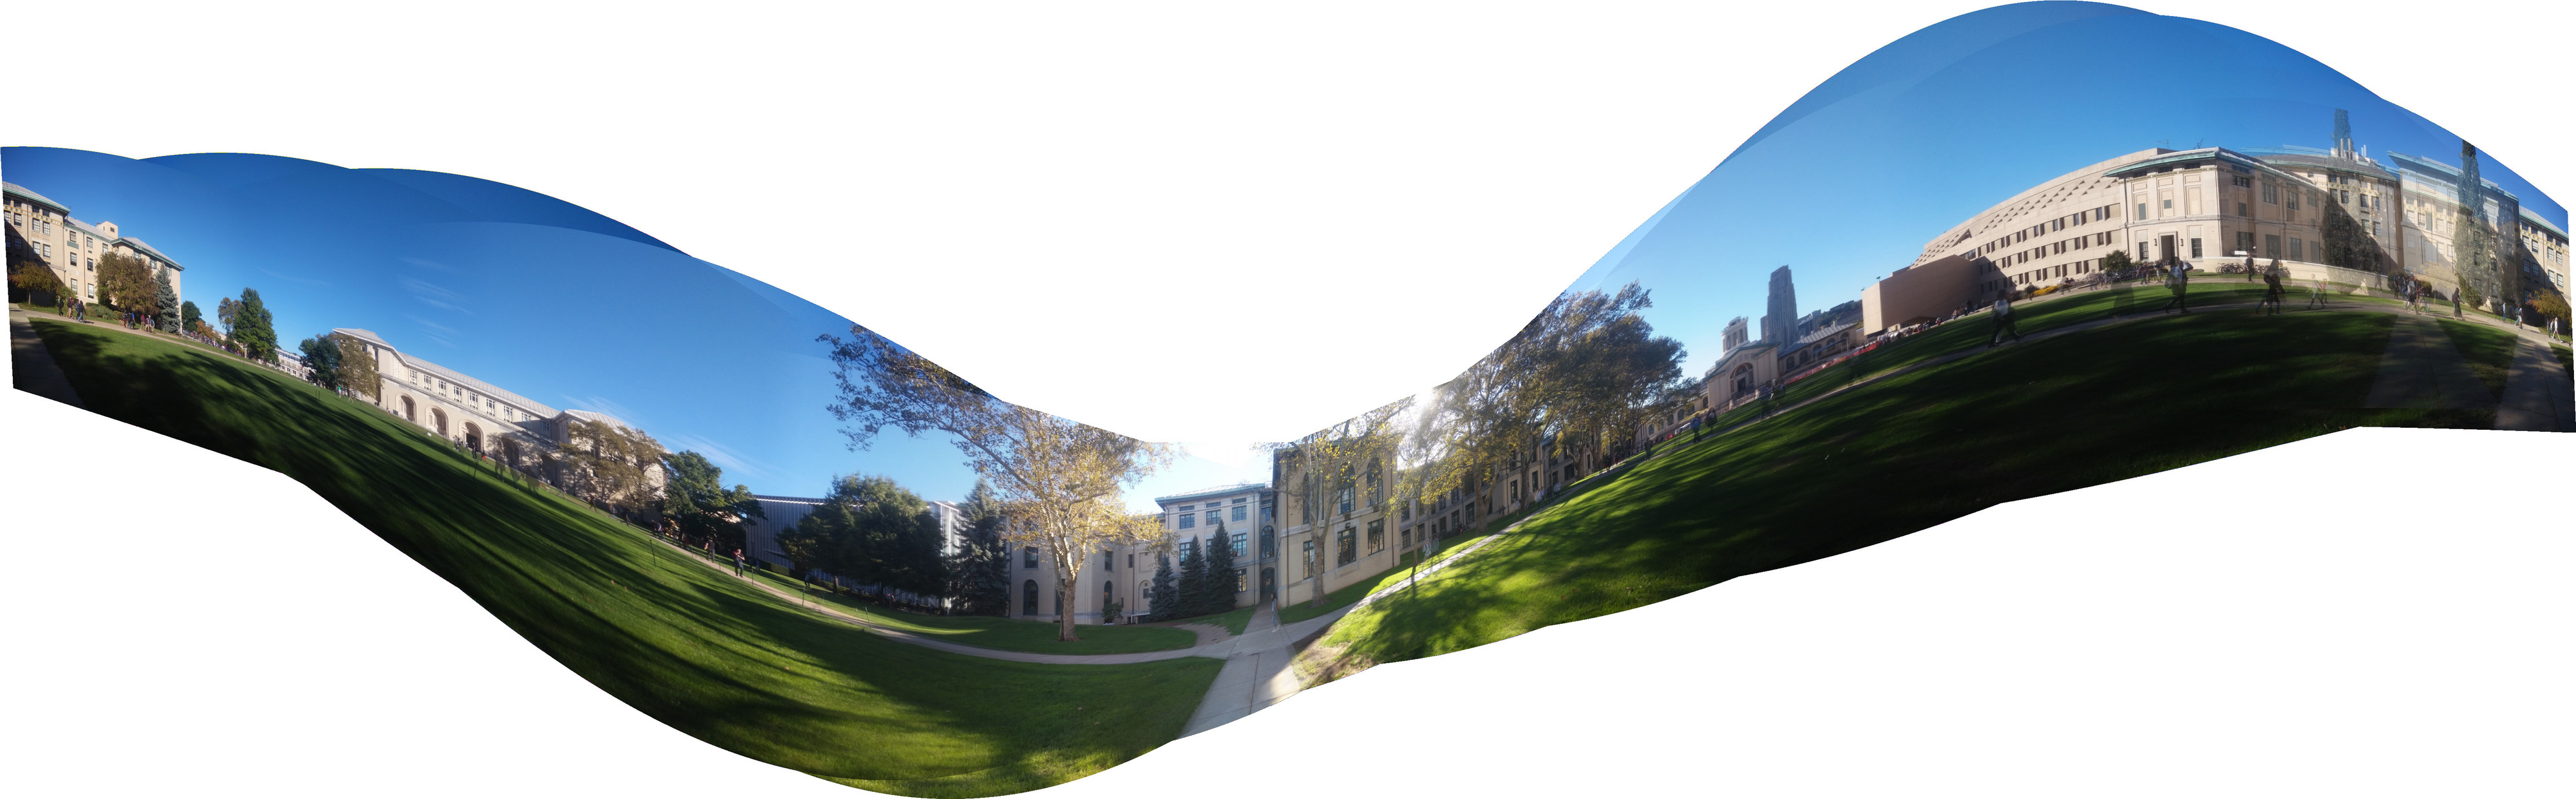
\includegraphics[width=1\textwidth]{res/CMU1-noestimate.jpg}
  \caption{CMU campus, directly stitched and then warped to cylinder}
\end{figure}

This is likely caused by our weak assumption on homography matrix.
A homography is estimated as a 3 by 3 matrix with the only
constraint being the scaling factor. However,
a homography is actually formed as:
\[ H_{1,2} = K_1R_1R_2^{-1}K_2^{-1}\]
where $K,R$ are intrinsic and rotation matrix of each camera.
From this formulation there should be a geometric constrain on each $H$,
which is not built into our initial estimation.
That's why the overall geometric structural is broken, although the matching pairs
are still well overlapped.

To overcome this problem, I estimated initial $K, R$ for each camera, from pairwise homographies.
Then, a global optimization is used to refine the parameters in $K, R$.
Finally, pairwise homographies are rebuilt from our refined $K, R$.

\subsubsection{Initial Estimation}
As suggested by \cite{focal}, focal length
can be roughly estimated from pairwise homographies. This is implemented in \verb|stitch/camera.cc|.
I used it to produce initial estimation of
focal length and assign it to each camera.

By assuming a rotation matrix for certain pivot image being identical,
other rotation matrices
can be estimated one by one using pairwise homography:
\[ R_1 = K_1^{-1}H_{1,2}K_2R_2\]

To reduce accumulated error,
I first construct a max-spanning tree by using
confidence of pairwise matches calculated in \secref{transform} (\verb|Stitcher::max_spanning_tree()|).
Then each time the most confidence pair is used to estimate
an unknown rotation matrix from a known one.

After obtaining a guess of $K$ and $R$ for each image,
pairwise homographies can be reconstructed and used to
stitch image together. A result is given below. Note that
the distortion is gone due to our constraints on the formulation
of pairwise homographies, but the quality is not satisfactory.
\begin{figure}[H]
  \centering
  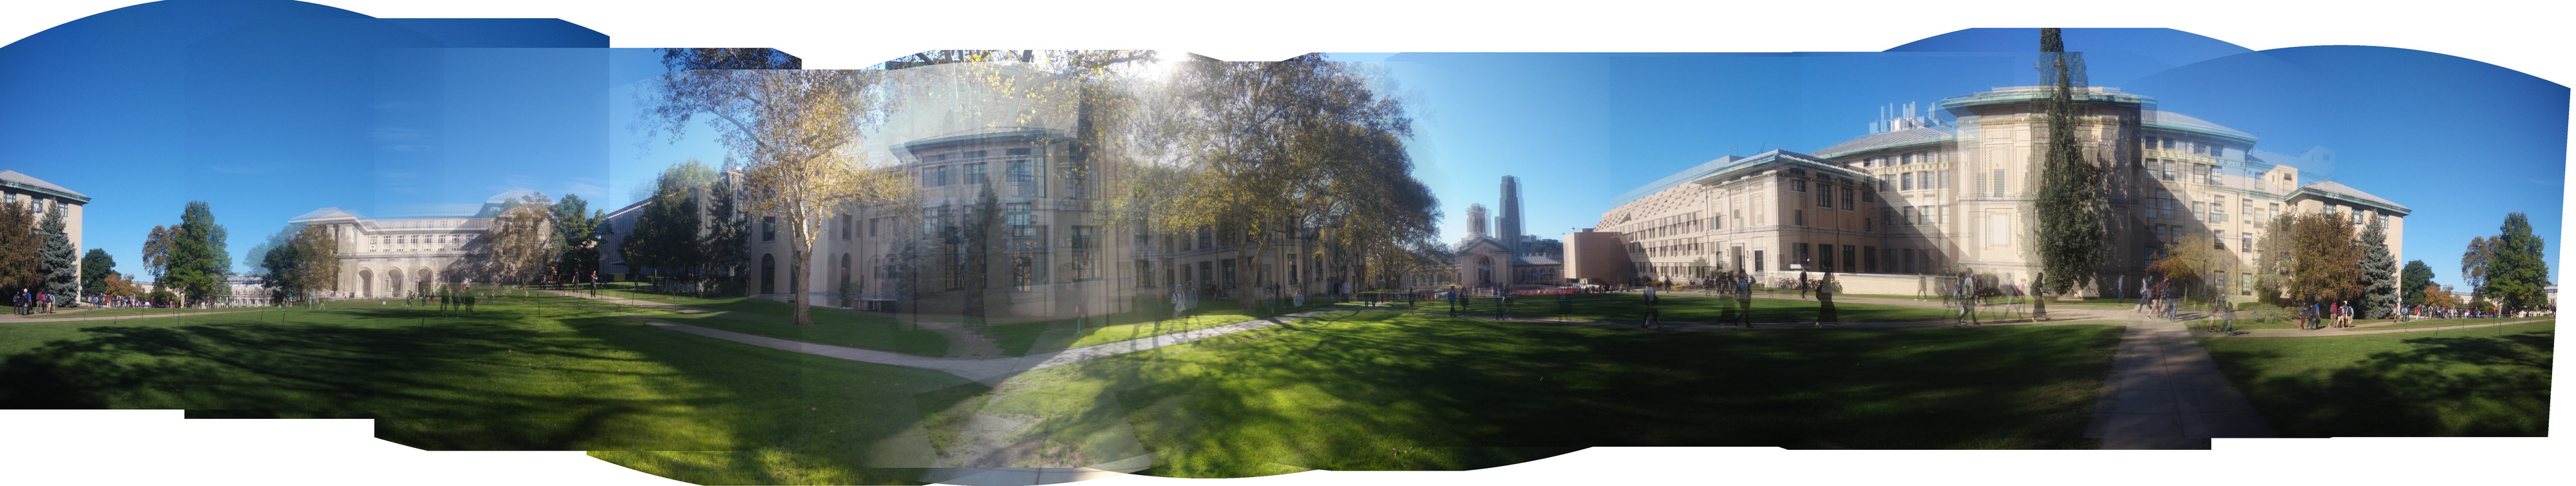
\includegraphics[width=\textwidth]{res/initial_camera.jpg}
  \caption{Initial guess of camera parameters}
\end{figure}

\subsubsection{Bundle Adjustment}

I implemented bundle adjustment in \verb|stitch/bundle_adjuster.cc|,
to globally optimize all the camera parameters.
The object is to minimize the sum of error of every matching pair of pixels.
The object function can be optimized in Levenberg-Marquardt algorithm
\footnote{\url{https://en.wikipedia.org/wiki/Levenberg–Marquardt_algorithm}}.
For simplicity, I used numerical differentiation to calculate
the Jacobian, although a closed-form formula is available,
as shown in \cite{panoramic-sift}.

During the optimization, the best params so far is kept.
The optimization ended when the error doesn't decrease
in the last 5 iterations.

After the optimization, the above panorama looks much better:
\begin{figure}[H]
  \centering
  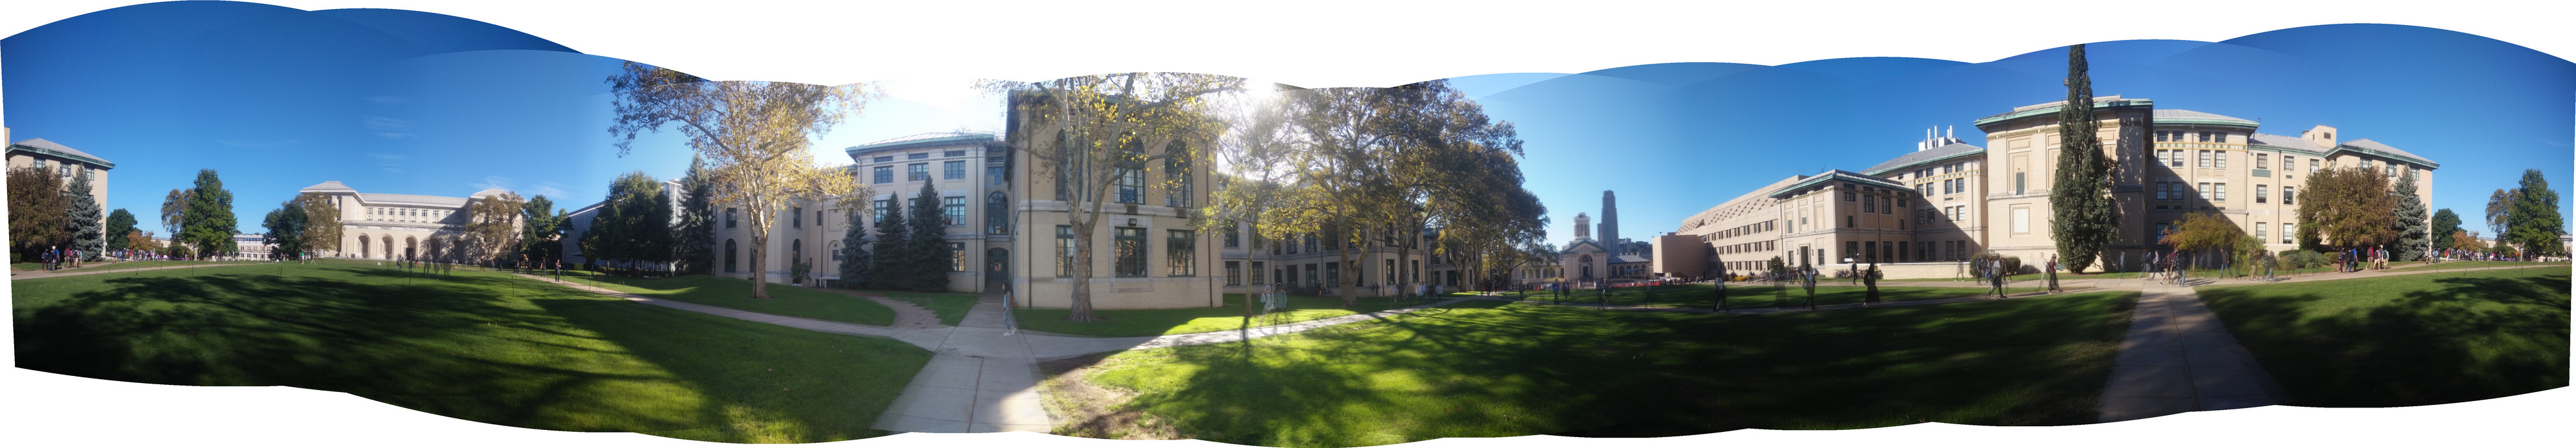
\includegraphics[width=\textwidth]{res/after-ba.jpg}
  \caption{After Bundle Adjustment}
\end{figure}

I noticed that in some hard cases, bundle adjustment cannot converge to a good result.
This is usually due to false matches or low-quality matches between images.
\cite{panoramic-sift} suggests incrementally adding images to the bundle adjuster,
which sounds reasonable but I don't have time to implement that for now.
Also, I think it'll also help to reject some matches if it is inconsistent with
the current bundle.

\subsubsection{Straightening}
As suggested by \cite{panoramic-sift}, the result of bundle adjustment
can have wavy effect, due to the unknown tilt angle.
By assuming all cameras have their $X$ vectors lying on the same plane,
we can estimate a $Y$ vector perpendicular to that plane
to account for the tilt and fix the wavy effect. This part
is implemented in \verb|stitch/camera.cc|.

See the following two images and notice the straight line on the grass
is corrected (it is actually a circle in the center of a soccer field).
\begin{figure}[H]
  \centering
  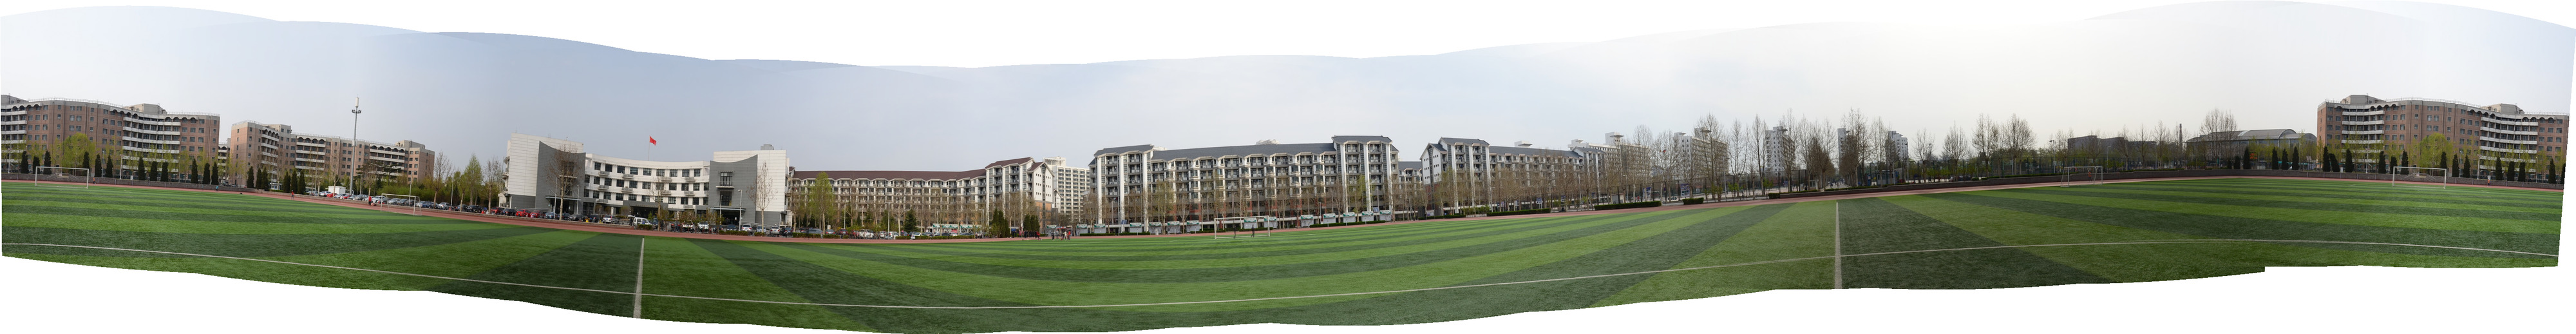
\includegraphics[width=\textwidth]{res/wavy.jpg}
  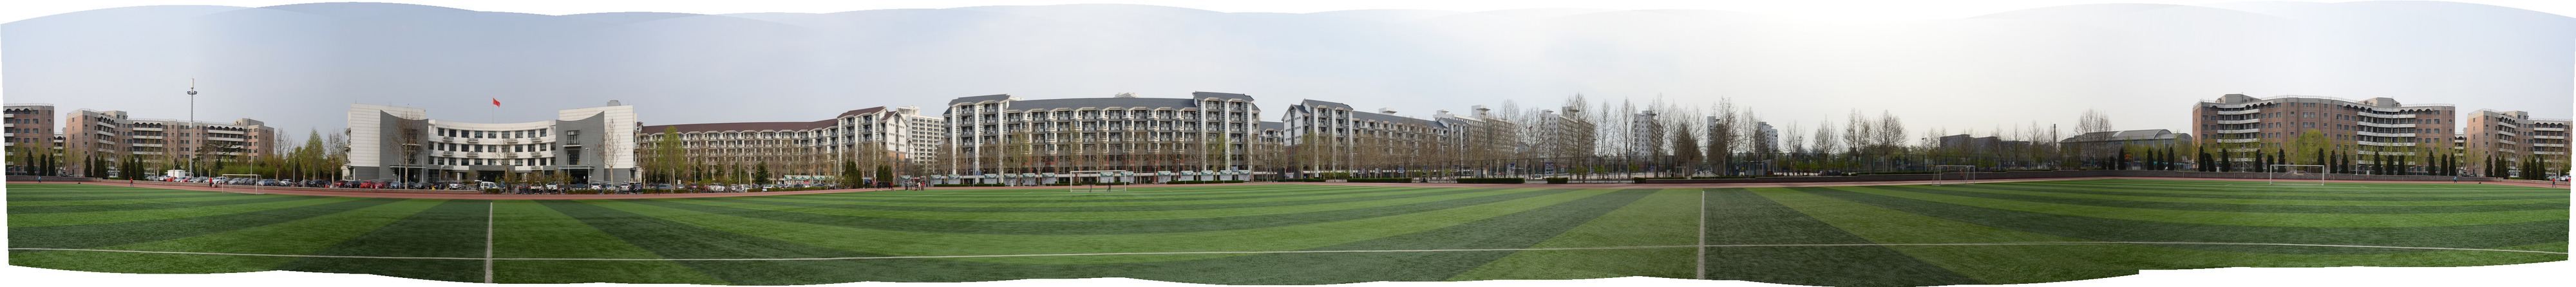
\includegraphics[width=\textwidth]{res/unwavy.jpg}
  \caption{Unstraightened and straightened result\label{fig:general-straighten}}
\end{figure}

